% 行列投影迭代法：Kaczmarz、扩展Kaczmarz与结果检验
\chapter{行列投影迭代法}
\label{sec:ls-row-projection}
\label{chap:row-projection-methods}

第~\ref{chap:stationary-iterations}章的定常迭代和第~\ref{chap:krylov-methods}章的Krylov方法，每轮都要用到整个矩阵，至少作一次矩阵乘向量。有些问题的数据却只方便逐行读取：观测按行陆续到达，或者矩阵太大，只能每次取出其中一行。这时自然的想法是每次只让一个方程成立，用一系列局部修正逐步逼近解。本章研究这种做法能求出什么解、何时收敛，以及方程不相容时应当怎样修改。

第~\ref{sec:ls-kaczmarz}节的Kaczmarz算法把当前解投影到所选方程的解超平面上，适用于相容方程；零初值时，它收敛到第~\ref{chap:linear-solution-selection}章的最小范数解。方程不相容时，各行没有公共解，单纯的行投影不会停在最小二乘解上。第~\ref{sec:ls-extended-kaczmarz}节的扩展Kaczmarz算法再用列投影估计右端中无法拟合的部分，把问题改写成相容方程后继续作行投影。第~\ref{sec:ls-row-projection-stopping}节说明两种算法分别用什么条件判断结果。

两种算法的推导都只用到超平面上的最短修正，即第~\ref{sec:ls-orthogonal-projection}节的正交投影；收敛分析用到伪逆、行空间与零空间的正交分解，以及第~\ref{chap:singular-value-decomposition}章中谱范数与最小正奇异值的刻画。本章$\bm A\in\mathbb R^{m\times d}$不必是方阵，两种算法都以$\bm A,\bm b$为输入、以$\bm x$为输出，投影中的残差和辅助向量只是内部状态。

\section{Kaczmarz算法}
\label{sec:ls-kaczmarz}

\term{Kaczmarz算法}（Kaczmarz method）每次只读取一行，把当前解修正到满足这一行的最近点。本节先由最短修正推导更新公式，再给出循环与随机两种选行方式，最后分析它对相容方程的收敛，并说明它为什么不能直接处理不相容方程。

\subsection{主要思想}

记第$i$行为$\bm a_i^\top$，其中$\bm a_i\in\mathbb R^d$是列向量。非零行的方程$\bm a_i^\top\bm x=b_i$的解集是以$\bm a_i$为法向量的超平面。给定当前点$\bm x_k$，要让新点$\bm x_k+\bm\delta$满足这一行，就要求
\[
 \bm a_i^\top\bm\delta=b_i-\bm a_i^\top\bm x_k ,
\]
其余的行暂不考虑。满足这个条件的修正有无穷多个，取其中欧氏范数最小的一个，使新点尽量少偏离当前点。

把任意修正分为沿$\bm a_i$的分量和与$\bm a_i$正交的分量：$\bm\delta=\gamma\bm a_i+\bm w$，$\bm a_i^\top\bm w=0$。行约束只涉及第一部分，给出$\gamma\lVert\bm a_i\rVert_2^2=b_i-\bm a_i^\top\bm x_k$；而由勾股关系，$\lVert\bm\delta\rVert_2^2=\gamma^2\lVert\bm a_i\rVert_2^2+\lVert\bm w\rVert_2^2$，在$\bm w=\bm0$时最小。于是得到Kaczmarz更新
\begin{equation}
 \bm x_{k+1}=\bm x_k+\frac{b_i-\bm a_i^\top\bm x_k}{\lVert\bm a_i\rVert_2^2}\,\bm a_i .
 \label{eq:ls-kaczmarz-update}
\end{equation}
代回所选行，$\bm a_i^\top\bm x_{k+1}=\bm a_i^\top\bm x_k+(b_i-\bm a_i^\top\bm x_k)=b_i$，这一行精确成立。分母$\lVert\bm a_i\rVert_2^2$来自法向量的长度，不是另外选取的步长；新点正是$\bm x_k$到该超平面的正交投影。

方程相容时，可以任取一个精确解$\bm y$观察距离的变化。由$\bm a_i^\top\bm y=b_i$，更新可写成$\bm x_{k+1}-\bm y=\bm P_i(\bm x_k-\bm y)$，其中$\bm P_i=\bm I-\bm a_i\bm a_i^\top/\lVert\bm a_i\rVert_2^2$是到$\bm a_i^\perp$的正交投影。勾股关系给出
\begin{equation}
 \lVert\bm x_{k+1}-\bm y\rVert_2^2=\lVert\bm x_k-\bm y\rVert_2^2-\frac{(b_i-\bm a_i^\top\bm x_k)^2}{\lVert\bm a_i\rVert_2^2}.
 \label{eq:ls-kaczmarz-distance}
\end{equation}
所以每一步到每个精确解的距离都不增，所选行的残差越大，距离减少得越多。距离减少并不意味着其他每一行的残差都减少：投影只照顾所选的一行，已经满足的行可能重新失配。

每次修正都是某个$\bm a_i$的倍数，留在行空间$\operatorname{range}(\bm A^\top)$中，所以$\bm x_k$的零空间分量始终等于初值的零空间分量。取$\bm x_0=\bm0$时，迭代始终在行空间中；若它收敛到一个精确解，这个解在行空间中，由定理~\ref{thm:ls-minimum-norm-representative}，它就是最小范数解。方程不相容时没有各行共有的解$\bm y$，式~\eqref{eq:ls-kaczmarz-distance}的论证不能照搬。

\subsection{算法实现}

\paragraph{初始化}
输入为可以逐行访问的$\bm A$和右端$\bm b$，输出为$\bm x$。超参数单独列出：初值$\bm x_0$，选行规则，残差容差$\mathrm{atol},\mathrm{rtol}$，以及最大更新次数$K$；要求最小范数解时取$\bm x_0=\bm 0$。若$\bm A=\bm0$且$\bm b=\bm0$，直接返回$\bm x=\bm0$。预先计算并保存各行的平方范数$\lVert\bm a_i\rVert_2^2$。零行且$b_i=0$的方程对任何$\bm x$成立，直接跳过；零行而$b_i\neq0$时方程$0=b_i$不可能成立，说明精确方程不相容，应报告这一点并停止，不能用式~\eqref{eq:ls-kaczmarz-update}除以零继续。初始化计数$k=0$，若$K=0$则直接取$\bm x=\bm x_0$并结束。

\paragraph{选行规则}
循环版本按$1,\ldots,m$的固定顺序重复遍历非零行，遍历一次称为一轮扫掠。随机版本每次按概率
\[
 p_i=\frac{\lVert\bm a_i\rVert_2^2}{\lVert\bm A\rVert_F^2}
\]
独立选取行$i_k$；零行的概率为零，不会被抽到。随机版本应记录选行序列，以便复算同一条轨迹。

\paragraph{行投影}
对所选行$i=i_k$，先计算行残差$s_k=b_i-\bm a_i^\top\bm x_k$，再计算修正长度$\gamma_k=s_k/\lVert\bm a_i\rVert_2^2$，然后更新$\bm x_{k+1}=\bm x_k+\gamma_k\bm a_i$。每完成一次行更新便把$k$加一。一次更新只读一行，不需要其他行的数据。

\paragraph{停止检查}
达到更新次数上限时立即结束并取当前$\bm x$，即使这一轮尚未扫完。在初始时和每轮完整扫掠后（随机版本则每隔预先规定的更新次数），用全部原方程计算原残差；若$\lVert\bm b-\bm A\bm x_k\rVert_2$不超过第~\ref{sec:ls-matrix-splitting}节的阈值$\mathrm{atol}+\mathrm{rtol}\lVert\bm b\rVert_2$，也结束并取当前$\bm x$。所选行的行残差为零只说明这一行成立，不能作为成功退出的依据。

\paragraph{算例}
先在第~\ref{chap:stationary-iterations}章的贯穿例上算两步，看清一次投影满足所选方程、却破坏另一个方程的现象；图~\ref{fig:ls-kaczmarz-projection-path}画出了这条路径。

\begin{example}[Kaczmarz算法的前两步]
\label{ex:ls-kaczmarz-two-steps}
用例~\ref{ex:ls-stationary-running-example}的方程，行$\bm a_1=(4,1)^\top$，$\bm a_2=(1,3)^\top$，平方范数分别为$17$和$10$，从$\bm x_0=\bm 0$出发按$1,2$的顺序投影。第一步第一行的残差为$1-0=1$，修正长度$\gamma_0=1/17$，得$\bm x_1=(4/17,\,1/17)^\top$，此时$4x_1+x_2=1$成立。

第二步第二行的残差为$2-(4/17+3/17)=27/17$，修正长度$\gamma_1=27/170$，得$\bm x_2=(4/17,1/17)^\top+\tfrac{27}{170}(1,3)^\top=(67/170,\,91/170)^\top$，第二个方程成立，第一个方程又不再成立。到$\bm x_\star=(1/11,7/11)^\top$的距离依次约为$0.643$、$0.595$、$0.320$。
\end{example}

再取一个两行接近平行的方程，连续算两轮扫掠，逐步记录全部原方程的残差。

\begin{example}[循环Kaczmarz的两轮扫掠]
\label{ex:ls-kaczmarz-two-sweeps}
取
\[
 \bm A=\begin{bmatrix}1&1\\1&2\end{bmatrix},\qquad \bm b=\begin{bmatrix}1\\2\end{bmatrix},\qquad \bm x_0=\bm0,
\]
精确解为$\bm x_\star=(0,1)^\top$，两行的平方范数为$2$和$5$。第一步选第一行，行残差为$1$，$\gamma_0=1/2$，得$\bm x_1=(1/2,1/2)^\top$，全残差$\bm b-\bm A\bm x_1=(0,1/2)^\top$。

第二步选第二行，行残差为$2-(1/2+2\cdot1/2)=1/2$，$\gamma_1=(1/2)/5=1/10$，得$\bm x_2=(3/5,7/10)^\top$，全残差为$(-3/10,0)^\top$：第二行满足后，第一行重新失配。

第二轮先选第一行，行残差为$-3/10$，$\gamma_2=-3/20$，得$\bm x_3=(9/20,11/20)^\top$，全残差为$(0,9/20)^\top$；再选第二行，行残差为$9/20$，$\gamma_3=9/100$，得$\bm x_4=(27/50,73/100)^\top$，全残差为$(-27/100,0)^\top$。

每一步都有一行的残差为零，但另一行的残差始终不为零，$\bm x_4$离$\bm x_\star$仍有约$0.604$的距离。是否停止要看每轮末全残差与容差的比较，不能把某次行残差为零当成成功。
\end{example}

\subsection{算法分析}

\paragraph{收敛性}
循环版本的收敛可以由投影的几何性质直接得到。下面$\bm A^\dagger$为伪逆（第~\ref{sec:ls-pseudoinverse}节），$\bm I-\bm A^\dagger\bm A$是到零空间$\ker\bm A$的正交投影。
\begin{theorem}[相容方程上循环Kaczmarz的收敛]
\label{thm:ls-kaczmarz-convergence}
设$\bm A\bm x=\bm b$相容且$\bm A\neq\bm 0$，令$\bm x_\star=\bm A^\dagger\bm b+(\bm I-\bm A^\dagger\bm A)\bm x_0$。按固定循环顺序遍历非零行时，$\bm x_\star$是方程的解，到它的距离逐步不增，且每完成一轮按与初值无关的因子$q<1$几何收缩，从而$\bm x_k\to\bm x_\star$。特别地，$\bm x_0=\bm 0$时极限是最小范数解$\bm A^\dagger\bm b$。
\end{theorem}
\begin{proof}
由$\bm A\bm A^\dagger\bm b=\bm b$（方程相容）与$\bm A(\bm I-\bm A^\dagger\bm A)=\bm0$，$\bm A\bm x_\star=\bm b$。由式~\eqref{eq:ls-kaczmarz-distance}取$\bm y=\bm x_\star$，到$\bm x_\star$的距离逐步不增。误差$\bm\varepsilon_k=\bm x_k-\bm x_\star$满足$\bm\varepsilon_{k+1}=\bm P_{i_k}\bm\varepsilon_k$；$\bm\varepsilon_0=\bm A^\dagger\bm A\bm x_0-\bm A^\dagger\bm b$在行空间中，而每个$\bm P_i$把行空间映到自身，所以$\bm\varepsilon_k$始终在行空间中。

一轮的误差映射是固定的$\bm K=\bm P_{i_p}\cdots\bm P_{i_1}$，其中$i_1,\ldots,i_p$是全部非零行。若行空间中的$\bm v$满足$\lVert\bm K\bm v\rVert_2=\lVert\bm v\rVert_2$，由式~\eqref{eq:ls-kaczmarz-distance}每次投影都没有缩短长度，各次投影都不改变向量，于是$\bm v$依次与每个非零行正交，$\bm v\in\ker\bm A\cap\operatorname{range}(\bm A^\top)=\{\bm 0\}$。取行空间的标准正交基排成$\bm Q$，令$\bm C=\bm Q^\top\bm K\bm Q$。由式~\eqref{eq:matrix-analysis-spectral-norm}，存在单位向量$\bm w$使$q=\lVert\bm C\rVert_2=\lVert\bm C\bm w\rVert_2$；$\bm K\bm Q\bm w$在行空间中，故$\lVert\bm C\bm w\rVert_2=\lVert\bm K\bm Q\bm w\rVert_2<\lVert\bm Q\bm w\rVert_2=1$。于是每完成一轮，误差长度至多乘以$q<1$，轮末误差几何地趋于零；轮内距离又不增，整个序列收敛到$\bm x_\star$。
\end{proof}
零初值使迭代始终留在行空间中，相容而解不唯一时选出最小范数解；任意初值的极限同样满足方程，但带着初值的零空间分量。

\paragraph{收敛速度与代价}
收敛速度受各行之间的夹角和访问顺序影响：行越接近两两正交，一轮去掉的误差越多。二维时，第一步之后误差已经平行于刚投影过的直线，此后每次投影都把误差长度乘以两条直线法向夹角的余弦$|\bm a_1^\top\bm a_2|/(\lVert\bm a_1\rVert_2\lVert\bm a_2\rVert_2)$。

在例~\ref{ex:ls-kaczmarz-two-steps}中，这个余弦为$7/\sqrt{170}\approx0.537$，距离从$0.595$降到$0.320$，比值正是这个数。例~\ref{ex:ls-kaczmarz-two-sweeps}的两行接近平行，余弦为$3/\sqrt{10}\approx0.949$，距离依次约为$1$、$0.707$、$0.671$、$0.636$、$0.604$，第一步之后每步只缩短约百分之五。两条直线越接近垂直，折线收拢得越快；越接近平行，路径就在狭窄的夹角里来回往复。

一次投影的成本为$O(\operatorname{nnz}(\bm a_i))$，其中$\operatorname{nnz}$表示非零元个数；全局残差检查另需一次完整的矩阵乘向量。

\begin{figure}[htbp]
  \centering
  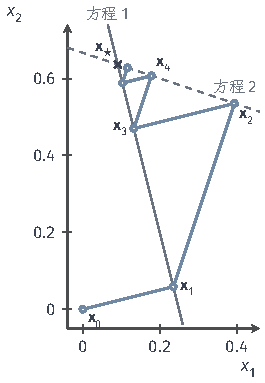
\includegraphics[width=44.81mm]{figures/01-basic-mathematics/03-vectors-matrices-and-multivariate-functions/tikz/c5-kaczmarz-projection-path/figure.pdf}
  \caption{循环Kaczmarz在贯穿例上的交替投影路径。实线为第一个方程$4x_1+x_2=1$的解集，虚线为第二个方程$x_1+3x_2=2$的解集；从$\bm x_0=\bm 0$出发依次垂直投影到两条直线上，折线连接精确计算的前六个迭代点并逐步收拢到交点$\bm x_\star$，图中标出前四个。坐标轴等比例，投影段与对应直线垂直。}
  \label{fig:ls-kaczmarz-projection-path}
\end{figure}

\paragraph{随机选行}
随机版本的投影公式不变，只是选行方式改为按$p_i$独立抽样，收敛结论因此是关于期望的。设方程相容，$\bm x_\star$如定理~\ref{thm:ls-kaczmarz-convergence}，误差$\bm\varepsilon_k$在行空间中。在给定$\bm\varepsilon_k$时对所选行求平均，由式~\eqref{eq:ls-kaczmarz-distance}，
\[
 \sum_{i=1}^mp_i\frac{(\bm a_i^\top\bm\varepsilon_k)^2}{\lVert\bm a_i\rVert_2^2}
 =\frac{\lVert\bm A\bm\varepsilon_k\rVert_2^2}{\lVert\bm A\rVert_F^2}
 \geq\frac{\sigma_r^2}{\lVert\bm A\rVert_F^2}\lVert\bm\varepsilon_k\rVert_2^2 ,
\]
其中$\sigma_r$是最小正奇异值，不等号来自定理~\ref{thm:ls-svd-singular-value-norms}对$\ker\bm A$正交补的下界。所以一步之后误差平方的平均至多是$(1-\sigma_r^2/\lVert\bm A\rVert_F^2)\lVert\bm\varepsilon_k\rVert_2^2$。选取概率与行的平方范数成正比，正是为了让这一平均化成$\lVert\bm A\bm\varepsilon_k\rVert_2^2$。

把这一步估计逐步叠加，得到$\mathbb E\lVert\bm\varepsilon_k\rVert_2^2\leq(1-\sigma_r^2/\lVert\bm A\rVert_F^2)^k\lVert\bm\varepsilon_0\rVert_2^2$；满列秩时这一结论由Strohmer与Vershynin给出\scite{math-strohmer2009randomized}。叠加时需要对此前各次选行的结果取条件期望，所用的随机变量与期望工具可参考\BookChapterRef{chap:random-variables}{卷七“随机变量与概率分布”章}。这里的结论是期望意义下的：单条轨迹上的误差每步不增，但不保证每一步都按这个因子缩小。

\paragraph{不相容情形}
不相容时情况不同。取$\bm A=(1,1)^\top$，$\bm b=(1,3)^\top$，未知量是标量，两行分别要求$x=1$和$x=3$。两行长度都为一，投影化为$x\gets b_i$，循环投影便在$1$与$3$之间往返，而最小二乘解是$\hat x=2$。随机选行时每一步$x$也只取$1$或$3$，所以仅改选行方式不能保证得到最小二乘解。不相容问题交给下一个算法处理。

\section{扩展Kaczmarz算法}
\label{sec:ls-extended-kaczmarz}

上一节的例子说明，方程不相容时，行投影总在各行的解之间来回，原因是右端含有任何$\bm x$都拟合不了的部分。\term{扩展Kaczmarz算法}（extended Kaczmarz method）先用列投影逐步取出这一部分，再对校正后的相容方程作行投影，从而把Kaczmarz算法推广到一般的最小二乘问题。

\subsection{主要思想}

由正交分解，$\bm b=\bm b_\parallel+\bm b_\perp$，其中$\bm b_\parallel\in\operatorname{range}(\bm A)$，$\bm b_\perp\in\ker(\bm A^\top)$，$\bm b_\perp$是不可拟合的部分。由第~\ref{sec:ls-ordinary-ls}节，最小二乘解就是相容方程$\bm A\bm x=\bm b_\parallel$的解，其中的最小范数解是$\bm A^\dagger\bm b$。$\bm b_\perp$事先未知，所以引入一个$m$维辅助向量$\bm z$去逼近它，再求解$\bm A\bm x=\bm b-\bm z$。

$\bm b_\perp$由$\bm A^\top\bm z=\bm0$刻画，即$\bm z$与每一列正交。记第$j$列为$\bm c_j$，要让当前$\bm z_k$满足一条齐次方程$\bm c_j^\top\bm z=0$，把上一节的最短修正原理用于这个超平面，得到列投影
\begin{equation}
 \bm z_{k+1}=\bm z_k-\frac{\bm c_j^\top\bm z_k}{\lVert\bm c_j\rVert_2^2}\,\bm c_j .
 \label{eq:ls-extended-kaczmarz-column}
\end{equation}
它相当于对相容方程$\bm A^\top\bm z=\bm0$作一次Kaczmarz投影。从$\bm z_0=\bm b$出发，每次减去的都是列的倍数，$\bm z$在$\ker(\bm A^\top)$中的分量始终是$\bm b_\perp$，变化的只是列空间中的部分$\bm z_k-\bm b_\perp$。

若校正量已知为$\bm z_k$，当前第$i$条目标方程是$\bm a_i^\top\bm x=b_i-(\bm z_k)_i$。沿用式~\eqref{eq:ls-kaczmarz-update}的推导，得到行投影
\begin{equation}
 \bm x_{k+1}=\bm x_k+\frac{b_i-(\bm z_k)_i-\bm a_i^\top\bm x_k}{\lVert\bm a_i\rVert_2^2}\,\bm a_i .
 \label{eq:ls-extended-kaczmarz-row}
\end{equation}

本章采用同步读取轮初状态的版本：$\bm z_{k+1}$和$\bm x_{k+1}$都由$(\bm z_k,\bm x_k)$计算，行更新不改用刚得到的$\bm z_{k+1}$。先更新$\bm z$、再用新$\bm z$更新$\bm x$的版本也可以使用，但两种时间顺序产生不同的数值轨迹，实现应与所用的收敛分析一致。这里采用Zouzias与Freris的随机版本\scite{math-zouzias2013randomized}。

误差有两个来源。列投影缩小$\bm z_k-\bm b_\perp$；行投影则是在右端仍受这一误差扰动时逼近$\bm A\bm x=\bm b_\parallel$。$\bm x_0=\bm0$且每步都沿行方向修正，保证$\bm x_k$始终在行空间中，最终选出最小范数代表。

\subsection{算法实现}

\paragraph{初始化与抽样}
输入为$\bm A,\bm b$，输出为$\bm x$；超参数为绝对容差$\mathrm{atol}$、相对容差$\mathrm{rtol}$和更新次数上限$K$。初始化内部状态$\bm x_0=\bm 0$，$\bm z_0=\bm b$，并计算各行、各列的平方范数作为抽样权重；若$\bm A=\bm 0$，直接返回最小范数解$\bm x=\bm 0$。每轮独立抽取行$i_k$和列$j_k$，概率分别为
\[
 p_i=\frac{\lVert\bm a_i\rVert_2^2}{\lVert\bm A\rVert_F^2},\qquad
 q_j=\frac{\lVert\bm c_j\rVert_2^2}{\lVert\bm A\rVert_F^2}.
\]
零行和零列的概率为零，不会被抽到，也就不会出现除以零。随机版本同样应记录抽到的行列序列。

\paragraph{列投影}
每轮先保存轮初状态$(\bm x_k,\bm z_k)$，再计算$\eta_k=\bm c_{j_k}^\top\bm z_k/\lVert\bm c_{j_k}\rVert_2^2$和$\bm z_{k+1}=\bm z_k-\eta_k\bm c_{j_k}$，即式~\eqref{eq:ls-extended-kaczmarz-column}。旧的$\bm z_k$保留给本轮的行更新使用。

\paragraph{行投影}
行投影仍读取旧的$(\bm z_k)_{i_k}$，计算
\[
 \gamma_k=\frac{b_{i_k}-(\bm z_k)_{i_k}-\bm a_{i_k}^\top\bm x_k}{\lVert\bm a_{i_k}\rVert_2^2},\qquad
 \bm x_{k+1}=\bm x_k+\gamma_k\bm a_{i_k},
\]
完成本轮后才以$(\bm x_{k+1},\bm z_{k+1})$同时替换旧状态。

\paragraph{停止检查}
在初始时和每隔预先规定的轮数，若
\[
\lVert\bm b-\bm z_k-\bm A\bm x_k\rVert_2\leq\tau_r
\quad\text{且}\quad
\lVert\bm A^\top\bm z_k\rVert_2\leq\tau_n ,
\]
或者已达到$k=K$，就终止并取$\bm x=\bm x_k$。阈值按各自的尺度取为$\tau_r=\mathrm{atol}+\mathrm{rtol}\lVert\bm b\rVert_2$与$\tau_n=\mathrm{atol}+\mathrm{rtol}\lVert\bm A\rVert_F\lVert\bm b\rVert_2$，后者的尺度来自$\lVert\bm A^\top\bm z_0\rVert_2=\lVert\bm A^\top\bm b\rVert_2\leq\lVert\bm A\rVert_F\lVert\bm b\rVert_2$。前一项检查$\bm x_k$对校正方程的拟合，后一项检查辅助向量与列空间的正交性；它们只是内部停止判据，$\bm z_k$和检查值都不作为输出。停止前再直接计算正规残差$\bm A^\top(\bm b-\bm A\bm x_k)$复核，不要求原残差$\lVert\bm b-\bm A\bm x_k\rVert_2$趋于零。

\paragraph{算例}
下面用上一节的不相容例算完两轮，看同步版本怎样使用轮初的校正量。

\begin{example}[扩展Kaczmarz算法的前两轮]
\label{ex:ls-extended-kaczmarz-two-rounds}
取$\bm A=(1,1)^\top$，$\bm b=(1,3)^\top$：唯一的列$\bm c_1=(1,1)^\top$的平方范数为$2$，两行的平方范数都为$1$。由正交分解，$\bm b_\parallel=2(1,1)^\top$，$\bm b_\perp=(-1,1)^\top$。初始$x_0=0$，$\bm z_0=\bm b=(1,3)^\top$。

第一轮列投影给出$\eta_0=(1+3)/2=2$，$\bm z_1=(1,3)^\top-2(1,1)^\top=(-1,1)^\top$，已经等于$\bm b_\perp$。行投影用的是旧的$\bm z_0=\bm b$，无论抽到哪一行，修正量都是$b_i-(\bm z_0)_i-x_0=0$，所以$x_1=0$不动。若行更新改用新的$\bm z_1$，这一步就会提前得到$x=2$；同步版本不这样做。

第二轮列内积为$-1+1=0$，所以$\bm z_2=\bm z_1=(-1,1)^\top$。若抽到第一行，$\gamma_1=1-(-1)-0=2$；若抽到第二行，$\gamma_1=3-1-0=2$。两种情况都得到$x_2=2$，此后不再改变。

最后核验：$\bm A x_2=(2,2)^\top=\bm b-\bm z_2$，$\bm A^\top\bm z_2=0$，两项停止检查值都为零。原残差$\bm b-\bm A x_2=(-1,1)^\top$不为零，残差平方和为$2$，正是$\min_x[(x-1)^2+(x-3)^2]$的最优值；原方程依然没有精确解，但$x_2=2$已经是最小二乘解。
\end{example}

\subsection{算法分析}

\paragraph{极限的含义}
列投影只减去列的倍数，保留$\bm b$的正交残差分量$\bm b_\perp$，同时缩小$\bm z_k-\bm b_\perp$；零初值和沿行方向的修正又使$\bm x_k$始终留在行空间中。当$\bm z_k$趋于$\bm b_\perp$时，行投影求解的就是相容方程$\bm A\bm x=\bm b_\parallel$，而它在行空间中的唯一解是$\bm A^\dagger\bm b$，所以这一构造指向最小范数最小二乘解。

\paragraph{列校正的收敛}
列投影是对相容方程$\bm A^\top\bm z=\bm 0$作Kaczmarz投影，初值为$\bm b$。由定理~\ref{thm:ls-kaczmarz-convergence}（对$\bm A^\top$应用），按固定循环顺序选列时，$\bm z_k$收敛到$\bm b$在$\ker(\bm A^\top)$上的正交投影，即$\bm b_\perp$，每轮按小于一的因子几何收缩。随机选列时，上一节的一步平均估计同样适用于$\bm z_k-\bm b_\perp$，它属于$\operatorname{range}(\bm A)$，平均缩小因子为$1-\sigma_r^2/\lVert\bm A\rVert_F^2$。

\paragraph{行迭代的误差递推}
令$\bm x_\star=\bm A^\dagger\bm b$，它满足$\bm A\bm x_\star=\bm b_\parallel=\bm b-\bm b_\perp$，故$b_i=\bm a_i^\top\bm x_\star+(\bm b_\perp)_i$。代入行投影，误差$\bm\varepsilon_k=\bm x_k-\bm x_\star$满足
\[
 \bm\varepsilon_{k+1}=\bm P_{i_k}\bm\varepsilon_k+\frac{(\bm b_\perp-\bm z_k)_{i_k}}{\lVert\bm a_{i_k}\rVert_2^2}\,\bm a_{i_k}.
\]
第一项是标准Kaczmarz的误差映射，第二项是校正误差带来的扰动，长度不超过$\lVert\bm z_k-\bm b_\perp\rVert_2/\lVert\bm a_{i_k}\rVert_2$。$\bm\varepsilon_k$始终在行空间中。

在循环版本中，把一轮行扫掠合起来，有$\lVert\bm\varepsilon_{\text{轮末}}\rVert_2\leq q\lVert\bm\varepsilon_{\text{轮初}}\rVert_2+\varphi$，其中$q<1$是定理~\ref{thm:ls-kaczmarz-convergence}中的因子，$\varphi$是本轮各步扰动长度之和，随$\bm z_k\to\bm b_\perp$趋于零。由这一递推，轮末误差有界；记其上极限为$L$，则$L\leq qL$，故$L=0$，即$\bm x_k\to\bm A^\dagger\bm b$。随机版本在规定的独立抽样下，期望平方误差以由$1-\sigma_r^2/\lVert\bm A\rVert_F^2$决定的几何速率趋于零\scite{math-zouzias2013randomized}，证明同样要用条件期望。这里不宣称每条轨迹的原残差逐步下降，例~\ref{ex:ls-extended-kaczmarz-two-rounds}中第一轮$x$就完全没有移动。

\paragraph{代价}
每轮访问一行、一列，并保存长度为$m$的$\bm z_k$，代价按访问的非零元个数计算；停止检查需要计算$\bm A\bm x_k$与$\bm A^\top\bm z_k$，各相当于一次完整的矩阵乘向量，所以只按规定间隔进行。数值敏感性仍受原问题小奇异值的影响：两种收缩因子都由$\sigma_r^2/\lVert\bm A\rVert_F^2$决定，它很小时收敛很慢。

\section{结果检验与停止准则}
\label{sec:ls-row-projection-stopping}

两种算法的目标不同，检验条件也不同。标准Kaczmarz求解相容方程，用原残差$\lVert\bm b-\bm A\bm x_k\rVert_2$检验，并且要用全部方程计算，不能用所选行的残差代替。扩展算法求解一般最小二乘，原残差趋于非零的$\bm b_\perp$，不能以它为零作为成功标准。

扩展算法的两项内部判据控制了正规残差。令$\bm r_k=\bm b-\bm A\bm x_k$，由$\bm r_k=\bm z_k+(\bm b-\bm z_k-\bm A\bm x_k)$得
\[
\lVert\bm A^\top\bm r_k\rVert_2\leq\lVert\bm A^\top\bm z_k\rVert_2+\lVert\bm A\rVert_2\,\lVert\bm b-\bm z_k-\bm A\bm x_k\rVert_2 ,
\]
所以两项都小时，最小二乘的正交条件$\bm A^\top\bm r=\bm 0$的偏离也小；停止前再直接计算$\bm A^\top(\bm b-\bm A\bm x_k)$复核。最小范数的要求则不由这些残差检验，而是由零初值和迭代始终留在行空间中保证。

两种方法的输出都只是当前的$\bm x$，达到次数上限不代表已经达到目标精度。比较速度时要区分一次行投影、一次完整扫掠和Krylov方法中含矩阵乘法的一次迭代：一次行投影只读一行，一轮扫掠才相当于一次矩阵乘向量，再把抽样权重的准备和全局残差检查计入总成本。结果的误差解释和方法选择分别见第~\ref{sec:ls-numerical-sensitivity}节和第~\ref{sec:ls-method-selection}节。

\FloatBarrier
\section{本章小结}
\label{sec:row-projection-summary}

本章回答了只能逐行或逐列访问数据时怎样求解线性方程。Kaczmarz算法每次只满足一个方程：由最短修正原理，更新沿所选行的法向进行，步长由行残差除以行的平方范数确定，新点是当前点到该超平面的正交投影。方程相容时，每一步到每个精确解的距离都不增；循环版本每轮按小于一的因子收缩，收敛到$\bm A^\dagger\bm b$加上初值的零空间分量，零初值时就是最小范数解。随机版本按行的平方范数抽样，期望平方误差以$1-\sigma_r^2/\lVert\bm A\rVert_F^2$为因子几何减小。

使用时要注意几个条件。行之间越接近平行，收敛越慢；零行对应非零右端说明方程不相容，必须单独处理；某一行的残差为零不说明求解完成。方程不相容时，标准Kaczmarz在各行的解之间往返，不论循环还是随机选行都不会停在最小二乘解上。

扩展Kaczmarz算法把右端分成可拟合与不可拟合两部分：列投影从$\bm z_0=\bm b$出发逼近不可拟合的$\bm b_\perp$，行投影求解校正后的相容方程$\bm A\bm x=\bm b-\bm z$。本章采用同步版本，两种投影都读取轮初状态；零初值保证极限是最小范数最小二乘解。

检验时，标准算法看全部方程的原残差；扩展算法看$\lVert\bm A^\top\bm z\rVert_2$与校正方程的残差，并复核正规残差，原残差最终非零是正常的。两种算法的最小范数性质都依赖零初值和行空间保持，不由残差判据保证。它们每步只读一行或一列，代价低，但收敛速度受$\sigma_r^2/\lVert\bm A\rVert_F^2$限制；误差解释与方法比较在第~\ref{chap:solution-error-regularization}章进行。
